\section{Szymon Niziński}
\label{sec: nizinskisz}



I added a photo of a Panda (see Figure~\ref{fig:panda1}).

\begin{figure}[h]
    \centering
    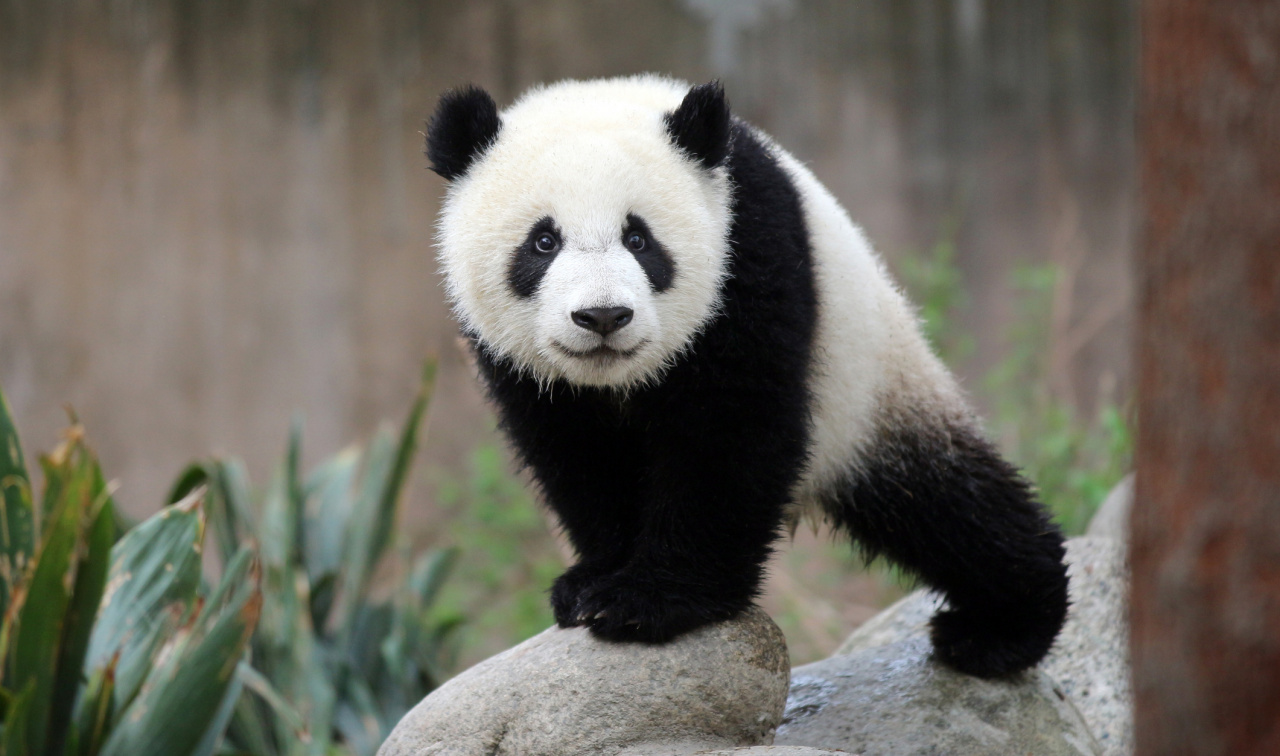
\includegraphics[width=0.9\textwidth]{pictures/panda.jpeg}
    \caption{This is a cute panda.}
    \label{fig:panda1}
\end{figure}

\subsection*{wyrażenie matematyczne}
We all know the famous Fermat' s Last Theorem:
\[ x^n + y^n = z^n \]
It states that no three positive integers a, b, and c can satisfy the equation if \( n > 2\).

\subsection*{tekst}

\textbf{Pierre de Fermat} - was a French mathematician who is given credit for early developments that led to infinitesimal calculus, including his technique of \textit{adequality}. In particular, he is recognized for his discovery of an original method of finding the greatest and the smallest ordinates of curved lines, which is analogous to that of differential calculus, then unknown, and his research into number theory. He made notable contributions to analytic geometry, probability, and optics. 

He is best known for his Fermat's principle for light propagation and his \textbf{\emph{Fermat's Last Theorem}} in number theory, which he described in a note at the margin of a copy of Diophantus' Arithmetica.

\subsection*{lista numerowana}
Top 5 potraw na Wigili:
\begin{enumerate}
    \item Barszcz z uszkami
    \item Ziemniaki z sosem grzybowym
    \item Pierogi z kapusta
\end{enumerate}

\begin{flushleft}
\vspace{0.5cm}
Wynik gry w Tic Tac Toe mozna zobaczyc tutaj (see Table ~\ref{tab:tablica})
\vspace{0.5cm}
\end{flushleft}

\subsection*{lista nienumerowana}
Zakres materiału na kolokwium z algebry:
\begin{itemize}
  \item[*] liczby zespolone
  \item[*] macierze
  \item[*] przestrzenie wektorowe
\end{itemize}

\subsection*{tabela}
\begin{table}[h]
    \centering
    \begin{tabular}{|c|c|c|}
        \hline
         X & X & O \\
        \hline
         O & X & O \\
        \hline
         X & O & X \\
        \hline
    \end{tabular}
    \caption{Tic Tac Toe}
    \label{tab:tablica}
\end{table}
